%================================================================
\section{Theory}\label{sec:Theory}
%================================================================

%----------------------------------------------------------------
\subsection{The Ising Model}\label{sec:ising theory}
%----------------------------------------------------------------
The Ising model is a binary value system where the variables of the model can take two values only, e.g. $\pm 1$ or 0 and 1. In statistical mechanics, the Ising model is used to model interacting magnetic dipole moments of atomic spins. The spins, denoted by $s$, are are arranged in a lattice with $L$ spin sites, allowing each spin to interact with its neighbors. The two dimensional square lattice Ising model exhibits a phase transition from a magnetic phase(a system with finite magnetic moment) to a phase with zero magnetization at a given critical temperature, called the Curie temperature, $T_C$. \cite{PROJising}

By simplifying the interaction between the spins to nearest neighbors only and assuming that the nearest neighbors have the same interaction strength, the Hamiltonian of the system can be defined as
\begin{equation}\label{eq:ising energy}
    H = - J \sum_{\ev{kl}} s_k s_l,
\end{equation}
where the spins $s=\pm 1$, $\ev{kl}$ indicates that the sum is over the nearest neighbors only, $J$ is a coupling constant expressing the strength of the interaction between neighboring spins. 

For $J>0$ it is energetically favorable for neighboring spins to be aligned, and the magnetic system will have a ferromagnetic ordering. Ferromagnetic materials exhibit a long-range ordering phenomenon where a given magnetic moment, through interactions between nearest neighbors, can influence the alignment of spins that are separated from the given spin by a macroscopic distance.
At temperatures below the Curie temperature, $T_C$, the ordering of spin states lead to a phenomenon called spontaneous magnetization. That is, the lattice has a net magnetization even in the absence of an external magnetic field. For temperatures $T\geq T_C$, however, the ferromagnetic property disappears as a result of thermal agitation. \cite{PROJising}

In the regression part of this study, we will consider the one-dimensional Ising model with nearest neighbor interactions on a chain of length $N$ with periodic boundary conditions, that is, spins at the boundary will have its nearest neighbors at the opposite boundary. In one-dimension \autoref{eq:ising energy} reduces to 

\begin{equation}\label{eq:ising 1D energy}
    H  = - J \sum_{j=1}^N s_j s_{j+1},
\end{equation}

This model does not exhibit any phase transition at finite temperature.



%----------------------------------------------------------------
\subsection{Linear Regression (revisited)}\label{sec:linreg theory}
%----------------------------------------------------------------
Linear regression is used to predict the value of a continuous dependent variable by simply computing a weighted sum of the input features. A study of three regression methods, namely, Ordinary Least Squares (OLS), Ridge, and Least Absolute Shrinkage and Selection Operator (Lasso), were carried out by the authors in \cite{PROJone}. For a detailed discussion of the aforementioned regression methods, as well as the mean squared error (MSE), coefficient of determination ($R^2$ score), bias and variance, please consult \autoref{sec:Appendix A} or \cite{PROJone}.

%--------------------------------------------------------------
\subsection{Logistic Regression}\label{sec:logreg theory}
%--------------------------------------------------------------
Some regression algorithms can be used for classification. Logistic regression can be used to classify instances into different classes by modelling the probability of a certain class or event existing. Unlike linear regression, the dependent  variables (also called responses or outcomes), $y_i$, is categorical, that is, $y_i$ are discrete and only take values from $K=0, ..., K-1$ (i.e. $K$ classes). The goal is to predict the output classes from the design matrix $X \in \R^{n\times p}$ made of $n$ samples, each of which carries $p$ features or predictors, with the primary goal being able to identify which classes unseen samples belong to. \cite{logreglec} \cite{Hands-onML}

We limit the following discussion to logistic regression as a binary classifier only, i.e. only two classes, here called positive and negative with corresponding outputs $y_i = 1$ and $y_i=0$.

\subsubsection{The Sigmoid Function}
In linear regression the output is the weighted sum of inputs. In logistic regression the output is not the weighted sum directly, we rather pass it through an activation function that can map any real value between 0 and 1. \cite{Hands-onML} The activation function is known as the sigmoid (or logit) function, and is given by

\begin{equation}\label{eq:sigmoid_func}
    \sigma (t) = \frac{1}{1+ e^{-t}} = \frac{e^t}{1+e^t}
\end{equation}
Note that $1-\sigma(t) = \sigma (-t)$

The sigmoid function is shown in \autoref{fig:logistic}.

\begin{figure}[H]
\begin{center}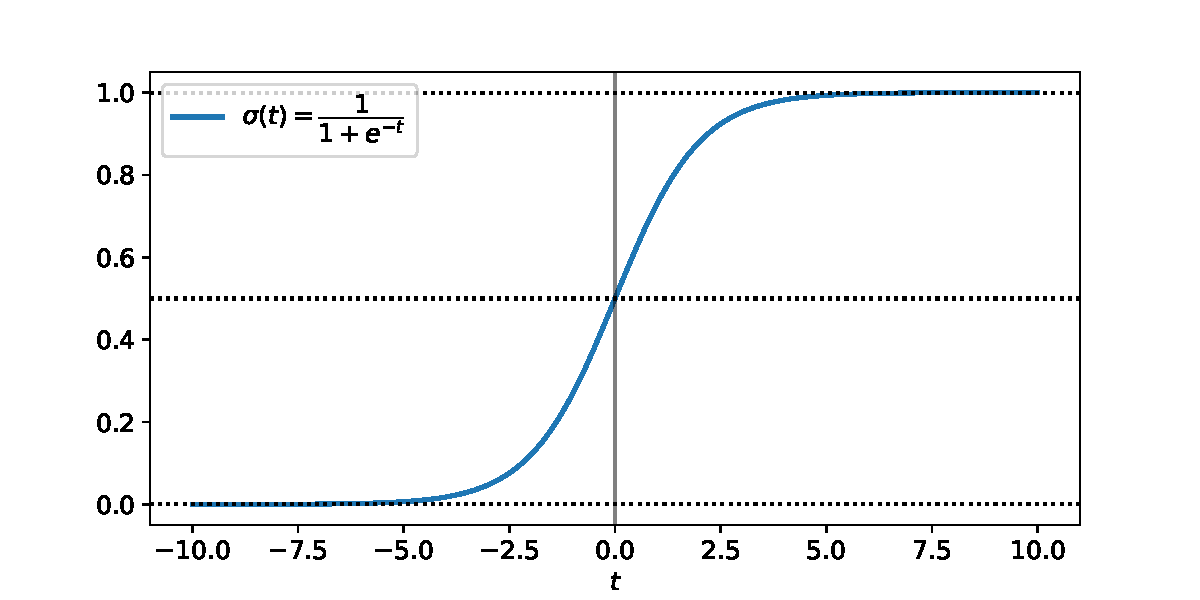
\includegraphics[scale=0.6]{latex/figures/logistic_function.pdf}
\end{center}
\caption{The sigmoid function is an activation function that can map any real value between 0 and 1.}
\label{fig:logistic}
\end{figure}

As seen in the figure, the value of the sigmoid function always lies between 0 and 1. The value is exactly 0.5 at $t=0$. Thus, 0.5 can be used as the probability threshold, $p$, to determine the classes. If $p \geq 0.5$ the instance $t$ belongs to the positive class ($y = 1$), or else we classify it as the negative class ($y = 0$). \cite{Hands-onML}

\subsubsection{The Logistic Regression Model}

A linear regression model can be represented by
\begin{equation}
    \bm{y} = \bm{\beta}^T \bm{X}
\end{equation}

The logistic regression models estimated probability is then
\begin{equation}
    \hat{p} = \sigma (\bm{\beta}^T \bm{X}),
\end{equation}

and the logistic regression model prediction is hence
\begin{equation}
\hat{y} = \begin{cases} 0 \quad \text{if } \hat{p} < 0.5 \\ 1 \quad \text{if } \hat{p} \geq 0.5 \end{cases} 
\end{equation}


\subsubsection{The Cost Function}
Like for linear regression, we define a cost for our model and the objective will be to minimize the cost.

The cost function of a single training instance can be given by

\begin{equation}\label{eq:logcost}
    C(\bm{\beta}) = \begin{cases} - \log(\hat{p}) &\quad \text{if } y=1 \\ - \log(1-\hat{p}) &\quad \text{if } y=0  \end{cases}
\end{equation}

\autoref{fig:logistic_cost} shows that this cost function makes sense.

\begin{figure}[H]
\begin{center}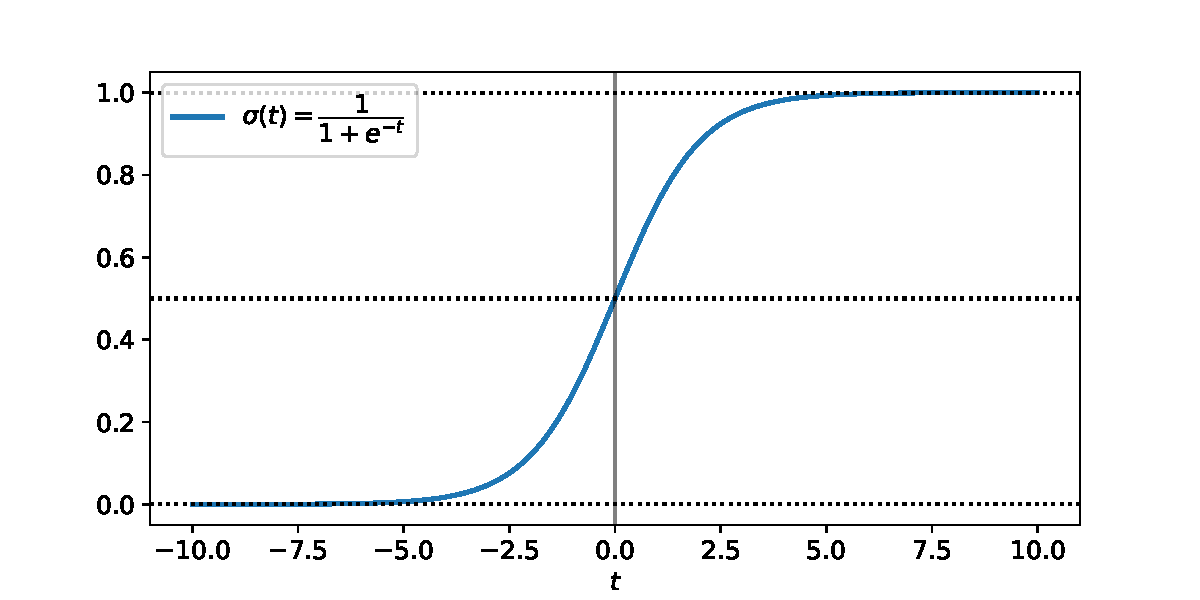
\includegraphics[scale=0.6]{latex/figures/logistic_cost_func.pdf}
\end{center}
\caption{The logistic cost function for a single training instance given by \autoref{eq:logcost}.}
\label{fig:logistic_cost}
\end{figure}

The objective of the cost function is to heavily penalize the model if it predicts a negative class ($y=0$) if the actual class is positive ($y=1$) and vice-versa. \cite{Hands-onML}

As seen in the above figure, for $C(\beta) = - \log(\hat{p})$ the cost nears 0 as $\hat{p}$ approaches 1 and as $\hat{p}$ nears 0 the cost goes toward infinity (that is, we penalize the model heavily). Similarly, for $C(\beta) = - \log(1 - \hat{p})$, when the actual value is 0 and the model predicts 0, the cost is 0, and the cost goes toward infinity as $\hat{p}$ approaches 1.

The total likelihood for all possible outcomes from a dataset $\mathcal{D} = \qty{\qty(y_i, x_i)}$ with binary labels $y_i \in \qty{0,1}$ and where the data points are drawn independently, can be defined in terms of the product of the individual probabilities of a specific outcome $y_i$ \cite{logreglec}:
\begin{equation}
    \hat{P} (\mathcal{D} | \bm{\beta}) = \prod_i \qty(\hat{p}\qty(y_i = 1 | x_i \bm{\beta}))^{y_i} \qty(1 - \hat{p}\qty(y_i = 1 | x_i \bm{\beta}))^{1-y_i} = \prod_i \hat{p}_i^{y_i} \qty(1 - \hat{p}_i)^{1-y_i},
\end{equation}
which should be maximized by the logistic regressor. Using the Maximum Likelihood Estimation (MLE) principle, we obtain the log-likelihood and the cost function over the whole dataset becomes, by arranging the sign so that it becomes a minimization problem,
\begin{equation}\label{eq:cross-entropy}
    J (\bm{\beta}) = - \sum_{i=1}^n \qty(y_i \log(\hat{p}_i) + (1-y_i) \log(1 - \hat{p}_i) )
\end{equation}
\autoref{eq:cross-entropy} is known in statistics as the cross-entropy.

There is no known closed-form solution to compute the value of $\bm{\beta}$ that minimizes this cost function. It is, however, convex, so Gradient Descent (or any other optimization algorithm) is guaranteed to find the global minimum (with the right learning rate and sufficient time). \cite{Hands-onML} 

The gradient of the cost function with regard to the model parameters $\bm{\beta}$ in compact matrix notation is given by
\begin{equation}\label{eq:logcost deriv}
    \nabla_{\bm{\beta}} J = -\bm{X}^T \qty(\bm{y} -\bm{\hat{p}})
\end{equation}

As with linear regression, we often supplement the logistic regressor with additional regularization terms to the cross-entropy, usually $L_1$ and $L_2$ regularization \cite{logreglec}.


The performance of a logistic regression model can be measured with the accuracy score, given by
\begin{equation}\label{eq:accuracy score}
    \text{Accuracy} = \frac{\sum_{i=1}^n I(t_i = y_i)}{n},
\end{equation}
where $I$ is the indicator function, 1 if $t_i = y_i$ and 0 otherwise, where $t_i$ represents the target and $y_i$ the outputs. A perfect classifier will have a score of 1.



%--------------------------------------------------------------
\subsection{Optimization and Gradient Methods}\label{sec:optim theory}
%--------------------------------------------------------------

\subsubsection{Gradient Descent}\label{sec:gradient descent}
Let $f\colon U\to\mathbb{R}$ be a function defined on a subset of $\mathbb{R}^n$. Suppose that $x\in U$ and that $f$ is differentiable in $x_0$. Then from the point $x_0$, the function $f$ has the steepest decrease in the direction along $-\nabla f(x_0)$. Hence, unless $x_0$ gives a minimum for $f$, given $\gamma_0 > 0$ small enough, we have that for $x_1 = x_0 - \gamma_0\nabla f(x_0)$, the inequality $f(x_1)\le f(x_0)$ holds. For all $n\in\mathbb{N}$, define
\begin{equation*}
    x_n = x_{n-1} - \gamma_{n-1}\nabla f(x_{n-1}),
\end{equation*}
where $\gamma_{n-1}>0$ is some number. If the $\gamma_{n}$ are chosen sufficiently small, the sequence $\{x_n\}_{n\in\mathbb{N}}$ converges to a local minimum. Larger $\gamma_{n}$ make the convergence faster.

\subsubsection{Newton-Raphson method}\label{sec:newton-raphson method}

This section is based on \cite[Section 5.6]{FVA}.

Let $A\subseteq\mathbb{R}^n$ and suppose that $f\colon A \to\mathbb{R}^n$ is a differentiable function. If $x_0\in A$, then for $x\in A$ “close” to $x_0$, the function $x\mapsto f(x_0)+Df(x_0)(x-x_0)$ is a good approximation of $f$. Assume that $f$ has a zero close to $x_0$. To try and find this zero, instead of solving $f(x)=0$, we solve the system of linear equations given by
\begin{equation*}
  f(x_0)+Df(x_0)(x-x_0) = 0.
\end{equation*}
If $Df(x_0)$ is invertible, we get the solution
\begin{equation*}
  x_1=x_0-(Df(x_0))^{-1}f(x_0).
\end{equation*}
We can hope that $x_1$ is even closer than $x_0$ to the actual zero of $f$. Repeating the process with $x_1$ instead of $x_0$, we find a new approximation
\begin{equation*}
  x_2=x_1-(Df(x_1))^{-1}f(x_1).
\end{equation*}
If we continue this for all $n\in\mathbb{N}$, we get a sequence $\{x_n\}_{n\in\mathbb{N}}$ where
\begin{equation*}
  x_n=x_{n-1}-(Df(x_{n-1}))^{-1}f(x_{n-1}).
\end{equation*}
Hopefully the sequence converges to a point $x=\lim_{n\to\infty}$ such that $f(x)=0$. This root-finding algorithm is called the \emph{Newton-Raphson method}.

In general Newton-Raphson is not guaranteed to work. Sufficient conditions are given in the Kantorovich theorem:
\begin{theorem}
  Let $f\colon U\to\mathbb{R}^n$ be a differentiable function defined on an open convex subset $U$ of $\mathbb{R}^n$. Assume that the Jacobian $Df$ of $f$ is Lipschitz continuous on $U$, i.e. that there exists an element $M\in\mathbb{R}$ such that
  \begin{equation*}
    \norm{Df(x)-Df(y)}\le M\norm{x-y}
  \end{equation*}
  for any $x,y\in U$.

Let $x_0\in U$ and suppose that $Df(x_0)$ is invertible. Find a number $K$ with $\norm{Df(x_0)^{-1}}\le K$, and assume that the closed ball $B\left(x_0,\frac{1}{KM}\right)$, with center in $x_0$ and radius $\frac{1}{KM}$ is contained in $U$. If
\begin{equation*}
  \norm{x_1-x_0}=\norm{Df(x_0)^{-1}f(x_0)}\le\frac{1}{2KM},
\end{equation*}
then $Df(x)$ is invertible for all $x$ in the open ball $B\left(x,\frac{1}{KM}\right)$. If we start Newton-Raphson in $x_0$, then all the points $x_n$ are contained in $B\left(x_0,\frac{1}{KM}\right)$ and the limit $x=\lim_{n\to\infty}x_n$ exists and satisfies $f(x)=0$.
\end{theorem}

%----------------------------------------------------------------
\subsection{Neural Network}\label{sec:dnn theory}
%----------------------------------------------------------------
Neural networks comprise a huge family of flexible function suitable of approximating nearly any function. Originally used as a simple model of the brain 
by McCulloch and Pitts in 1943(Siter), the field of neural networks has proved to be extremely useful in the world of modelling and machine learning. Today, the progress is still going strong, with application in a vast number of fields and many different flavors of neural networks

\subsubsection{Architechture of the Feed-Forward Neural Network}
In this project, we focus on the feed-forward neural network, hereafter referred
to simply as neural network. A neural network is in essence a real-valued function that may take number of inputs and outputs. It's behaviour is completely determined by its architecture, which is comprised of hidden layers.

A hidden layers is a set of nodes that relates to the emitted values of the 
previous hidden layer, or the inputs, it case it is the first hidden layer in the 
network. For the i'th node in the first hidden layer, its activation is 
calculated as
\begin{equation}\label{eq:activation}
    z^1_j = \sum_{i=1}^N W^1_{ji}x_j + b^1_j,
\end{equation}
where $N$ is the number of inputs $x$, $W^1$ is a matrix of the weights connecting the inputs to the first hidden layer, and $b^1$ is a constant bias term added to the activation. Taking the activation as the output of the first hidden layer, \autoref{eq:activation} defines a method of feeding information to the next hidden layer as well, and ultimately through the entire network. However, it can easily be seen from the equation that the feeding of information from one layer to another is a affine transformation. Since a affine transformation of a affine transformation is a affine transformation in itself, adding more layers to a network fails in making a more complex model. To avoid this collapse of 
layers, we need to introduce a non-linear function $f^1$ to the activation before 
passing it to the next layer
\begin{equation}\label{eq:non_linear}
    a^1_j = f^1(z^1_j)
\end{equation}

Non-linear functions used are typically sigmoid, $\tanh$ or the Relu, and enables neural network of becoming powerful and flexible models.

\subsubsection{Backward Propagation}
To evaluate how good a neural network performs on data, some kind of 
cost function is consulted

\begin{equation}\label{eq:cost}
    C(y, \tilde{y}) = \sum_{i=1}^N c(y_i, \tilde{y_i}) 
\end{equation}
Where the sum is over $N$ data-points, $y_i$ is the target of the i'th data point,
and $\tilde{y_i}$ is the accompanying prediction of the network given by $\tilde{y_i} = NN(X_i)$. $c$ is typically he square loss for regression

\begin{equation}\label{eq:square_loss}
    c(y_i, \tilde{y_i}) = (y_i - \tilde{y_i})^2,
\end{equation}

and cross entropy for binary classification
\begin{equation}\label{eq:square_loss}
    c(y_i, \tilde{y_i}) = y_i\log(\tilde{y_i}) + (1 - y_i)\log(1 - \tilde{y_i}),
\end{equation}

For a untrained neural network, the weights $W$ connecting all the layers are typically initialized in random fashion, popularly as $W \sim N(0,1)$, and the biases $b$ set to a small number such as $0.01$. 

To improve the model from the initial random state, we would like to minimize the cost function with respect to the weights. As the neural network is a very complex function, and not even a convex problem where are minima are global minima, the optimal weights can not be found by $\frac{dC}{dW^l_{ij}} = 0$. Instead, we resort to using gradient decent methods.

To compute the gradient $\frac{dC}{dW^l_{ij}}$, we use the chain rule repeatedly to produce an expression that keeps track of how the variation of the cost function propagates backward in the neural network, so-called backward propagation.

To start, we calculate the derivative of the cost function with respect to the weights of the last hidden layer:

\begin{equation}\label{eq:gradient}
    \frac{dC}{dw^L_{ij}} = \frac{dC}{da_j^L} \frac{da_j^L}{dw^L_{ij}} 
    = \frac{dC}{da_j^L} f'(z_j^L) \frac{dz^L_j}{dw^L_{ij}} = \frac{dC}{da_j^L} f'(z_j^L) a^{L-1}_i
\end{equation}
where we have used the chain rule repeatedly and the definition of the activation \autoref{eq:activation}.

Defining $\delta_j^L = \frac{dC}{da_j^L} f'(z_j) = \frac{dC}{dz_j^L}$, we can now look at the derivative of an arbitrary layer $l$:

\begin{equation}\label{eq:Backward}
   \delta_j^l = \frac{dC}{dz^l_j} = \sum_k \frac{dC}{dz^{l+1}_k} \frac{dz^{l+1}_k}{dz^{l}_j} = \sum_k \delta_k^{l+1} \frac{dz^{l+1}_k}{dz^{l}_j}
   = \sum_k \delta_k^{l+1} w_{kj}^{l+1}f'(z^l_j)
\end{equation}
This enables us to calculate the error propagation to an arbitrary layer, and we can calculate the gradient from \autoref{eq:gradient}. The update rules for a standard GD thus becomes

\begin{equation}\label{eq:grad step}
    w^l_{jk} \rightarrow w^l_{jk} - \mu \delta_j^l a_k^{l-1}  
\end{equation}
\begin{equation*}\label{}
    b^l_{j} \rightarrow b^l_{j} - \mu \delta_j^l 
\end{equation*}
where $\mu$ is the learning rate.

\subsubsection{Regularization}

Neural networks quickly grow in complexity as you increase the number of hidden layers and number of neurons for each layer. one must take care not to overfit the networks. A common approach is to add the L2-norm of the weights to the cost function, in the same spirit as the ridge regression:
\begin{equation*}
    C(y, \tilde{y}) = \sum_i(y_i - \tilde{y_i})^2 + \lambda \sum_{ijl}{w^l_{ij}}^2
\end{equation*}
This changes the update rule for the weights to
\begin{equation}\label{eq:grad step}
    w^l_{jk} \rightarrow w^l_{jk} - (\mu \delta_j^l a_k^{l-1} + \lambda'w^l_{jk}) 
\end{equation}
where $\lambda' = \mu \lambda$.
